\graphicspath{{chapters/07/images/}}
\chapter{Introduction}

\section{Systems}
A system is a set of integrated and interacting \emph{components} or \emph{entities} that form a whole with definite boundaries and surrounding environment.
It has a goal to achieve by performing one or more functions or tasks.
Systems can be aggregated into a \textbf{\emph{hierarchy}}.
A system at a given level of detail can be a component of another at a higher level of detail.

\begin{multicols}{2}
  \begin{itemize}
    \item A complex (non-linear) system is a system that does not satisfy the principle of superposition: the behaviour of the system cannot be inferred from the behaviour of its components.
    \item A dynamical system is a system where fixed rules define the time dependencies of the system in a geometrical space.
      Dynamical systems have a space and time dimension because they change their characteristics over time.
      Picking snapshots of the system at different time points, different configurations of the system (data) are observed
  \end{itemize}
\end{multicols}

  \subsection{Configuration}
  A configuration or state of the system refers to the current condition of the system and stores enough information to predict its next move.
  A state is characterized by the position of its components in a geometrical space and by the values of the attributes of its components like concentration or number of each elements involved.
  Systems change their state over time by changing the location of some of their components or changing the attributes of some of their components.
  Some particular configuration are:

  \begin{multicols}{2}
    \begin{itemize}
      \item Steady state: some of the attributes of the system will no longer change in the future.
      \item Transient state: time needed to reach the steady state.
    \end{itemize}
  \end{multicols}


  \subsection{Determinism, nondeterminism and stochasticity}

  \begin{multicols}{2}
    \begin{itemize}
      \item Deterministic systems always react in the same way to the same set of stimuli.
        These systems are completely determined by the initial state and the input set.
        The essence of deterministic systems is that each event is causally related to previous events and choices are always resolved in the same way in the same context.
      \item Nondeterministic systems are systems in which multiple different outcomes can be generated from the same input in different observation, and so the output cannot be predicted from the input.
      \item Stochasticity is the quality of lacking any predictable order or plan and stochastic systems possess some inherent randomness.
        It is possible to transform a nondeterministic system into a stochastic one by attaching probabilities to the selection points so that nondeterministic choices are turned into probabilistic choices.
    \end{itemize}
  \end{multicols}


  \subsection{Computational complexity}
  Complexity arises when interacting components self-organize to form evolving structures that exhibit a hierarchy of emergent system properties.
  An emergent behaviour can be originated by a collection of components that interact in the absence of a centralized point of control to produce something that has not been designed or programmed in the system construction or evolution.
  Computational complexity is the amount of resources, measured as a function of the size of the input, needed to execute an algorithm.
  It is divided into:

  \begin{multicols}{2}
    \begin{itemize}
      \item Computational space complexity: the amount of memory needed during the execution
    \item Computational time complexity: the number of instructions to be executed.
    \end{itemize}
  \end{multicols}


\section{Models}
A \emph{representation} is a set of symbols used to convey information and knowledge about a system.
It is either physical as a cell or an ecosystem, or artificial as a computer network or an economic market.
An abstraction is a representation that ignores some aspects of a system which are not of interest for the current investigation.
A \emph{model} is an abstraction of a system.
A model has its own interacting components that are characterized by the attributes that are under investigation.
The set of all the attributes in a model is the experimental frame.

\begin{multicols}{2}
  \begin{itemize}
    \item A dynamic model aims at predicting the behaviour of the system in time and space through what if analysis.
      What if analysis investigates how a change in some attributes affects the behaviour of the modelled system.
    \item A computational model is a model that can be manipulated by a computer to observe properties of the corresponding system.
  \end{itemize}
\end{multicols}

\begin{figure}[H]
  \centering
  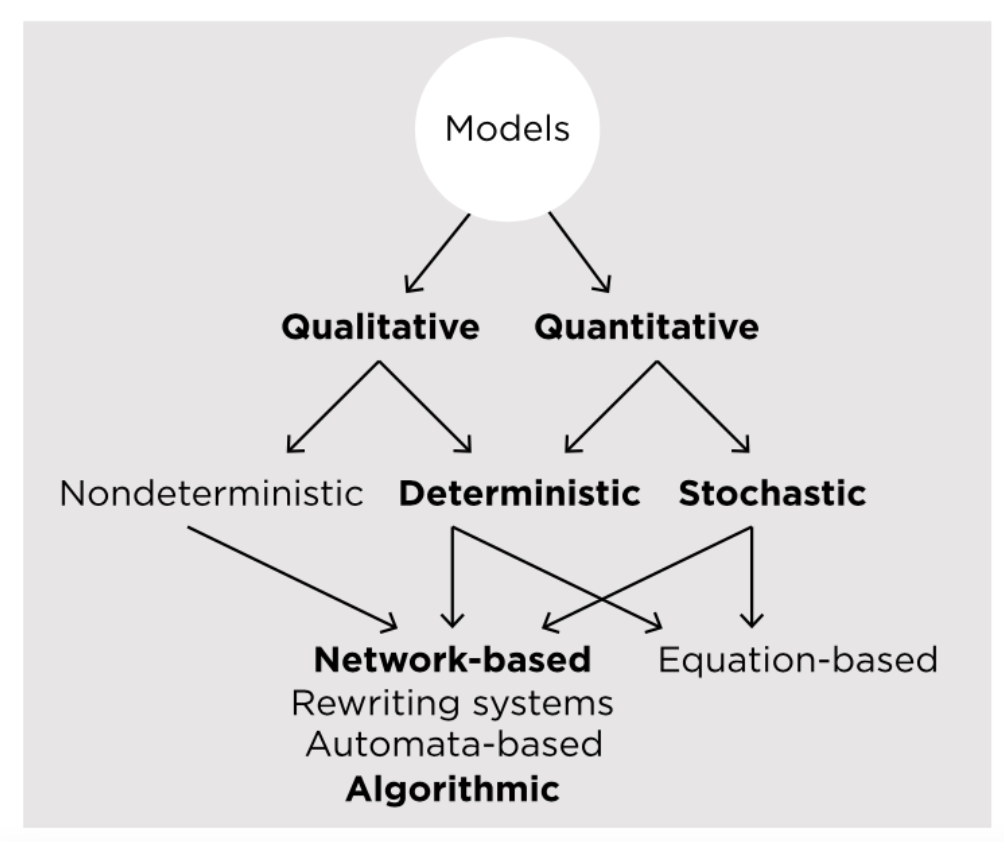
\includegraphics[width=0.6\textwidth]{scheme_model.png}
  \caption{From a model to methods}
\end{figure}

  \subsection{Checking the validity of a model}
  \emph{Validity} is a fundamental property of models and witnesses the capacity of a model of making good predictions.
  Assessing the validity of a model is a fundamental step to predict the behaviour of the system of interest.
  Assume that $M$ is a model for the system $S$ and $\underline{M}$ is the modelling process.
  Let $s(t)$ and $m(t)$ be the state of the system and of the model at time $t$, and $f_s$ and $f_m$ the state transition functions of the system and of the model respectively.
  Finally, let $I_s(t)$ and $O_s(t)$ be the input and output of the system at time $t$.
  Similarly, the input and output are defined also for the model $I_m(t)$ and $O_m(t)$.
  Going from one state to the there there is a function for the system and one for the model.
  In particular in a mathematical model $f_m$ is integrated to investigate the transition phase, while for the real system $f_s$ is knot known.
  Because of this the model needs to be I/O validated known input and output are used to investigate it, where input and output are generalized concepts.
  For example, an input can be any perturbation of the system, while an output any observable property causally related to the input.
  Now a model $M$ can be said to be valid for a system $S$ if:

  $$f_m(\underline{M}(s(t_0))) = \underline{M}(f_s(s(t_0))) = m(t_1)$$

  \begin{figure}[H]
    \centering
    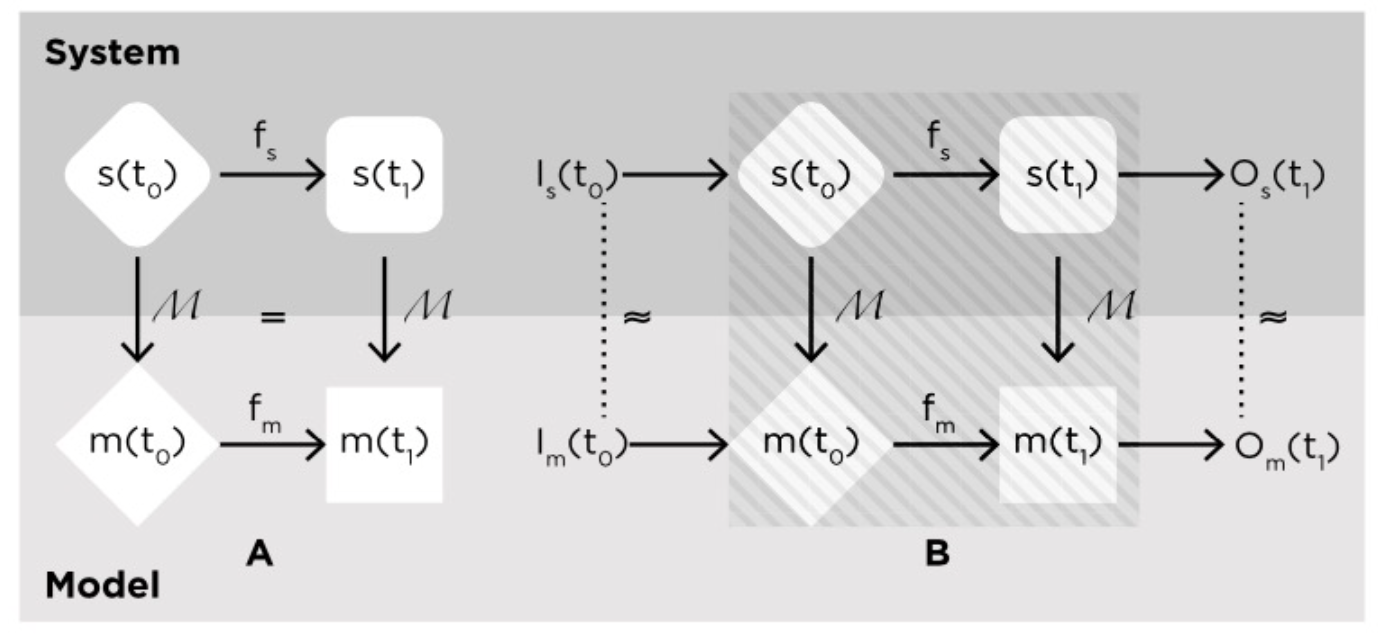
\includegraphics[width=0.7\textwidth]{validation.png}
    \caption{Validation}
    \end{figure}
  \noindent

  An I/O validity check can be performed by comparing data-set from the system and from the model.
  This checking process could cause overfitting:

  \begin{multicols}{2}
    \begin{itemize}
      \item A model is well tuned to a specific dataset used to build the model.
      \item It performs poorly on other datasets.
    \end{itemize}
  \end{multicols}

    \subsubsection{Cross validation}
    Cross validation is a process that checks overfitting by testing the model on data sets different from the ones used to build and calibrate or train the model.
  These concepts, even if usually referred to computational models, may apply to general models or representations of a system.

  \subsection{Building a model}
  The first step to build a model is to define:

  \begin{multicols}{2}
    \begin{itemize}
      \item The system to be modelled.
      \item The property of interest of the system.
      \item The expected output.
      \item The objective of the model.
    \end{itemize}
  \end{multicols}

  \begin{figure}[H]
    \centering
    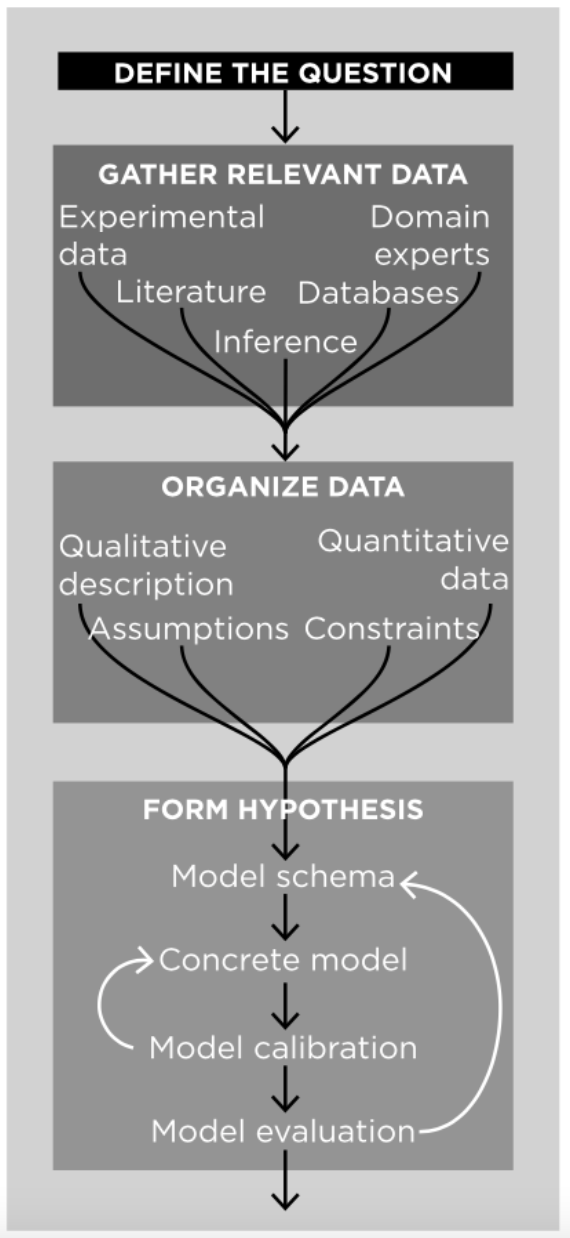
\includegraphics[width=0.3\textwidth]{workflow.png}
    \caption{Workflow}
  \end{figure}

  After defining these things them model needs to be built and calibrated, so to check if it can recapitulate data.
  If it does not, the model can be wrong or some parameters need to be tuned.
  It is important to note that different parameters can lead to dramatic changes in dynamics, like for example, in the Lotka-Volterra model in figure \ref{fig:Volterra}.
  It can be noted how this example shows periodic oscillation, with the same amount of preys and predators, on the left, while on the right, after parameter change, it shows higher peaks and a lower predator presence.

  \begin{figure}[H]
    \centering
    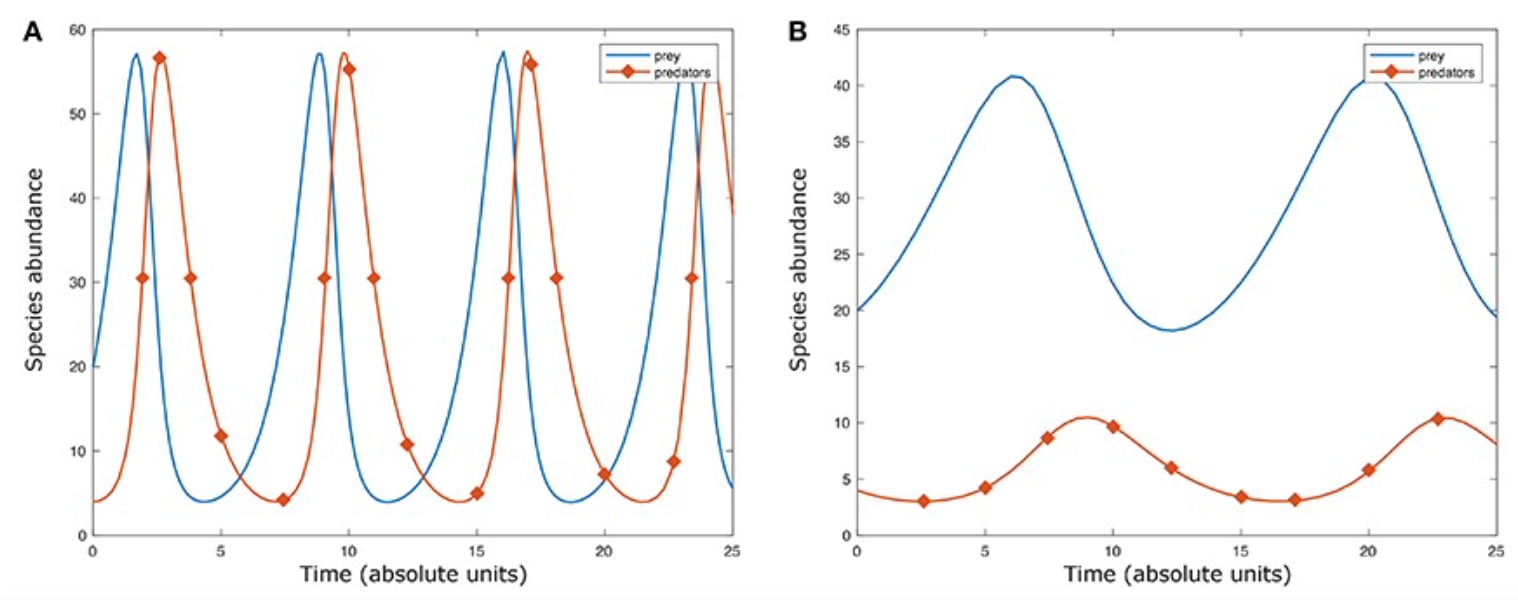
\includegraphics[width=\textwidth]{volterra.png}
    \caption{Lotka-Volterra model}
    \label{fig:Volterra}
  \end{figure}
